\section{Intensity correlations}

\begin{figure}[!ht]
    \centering
    \subfloat[\label{fig:simple_optical_model:a}]{
        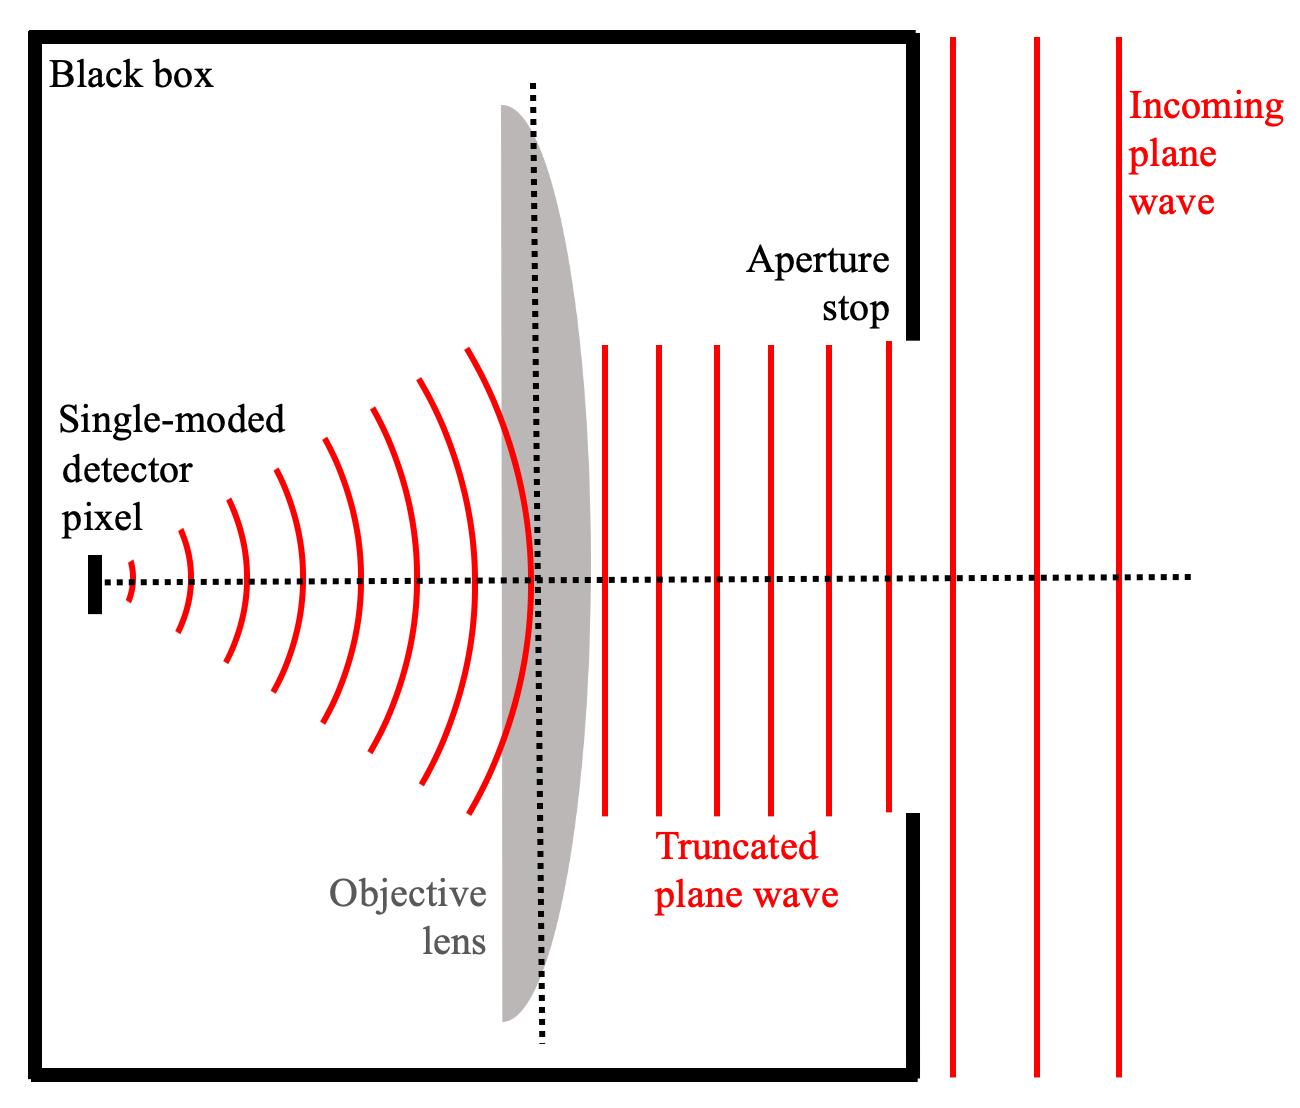
\includegraphics[width=0.40\linewidth, trim=0mm 0mm 0mm 0mm, clip=true]{WhiteNoiseCorrelations/Figures/simplified_optics_wave.png}
        }
    \subfloat[\label{fig:simple_optical_model:b}]{
        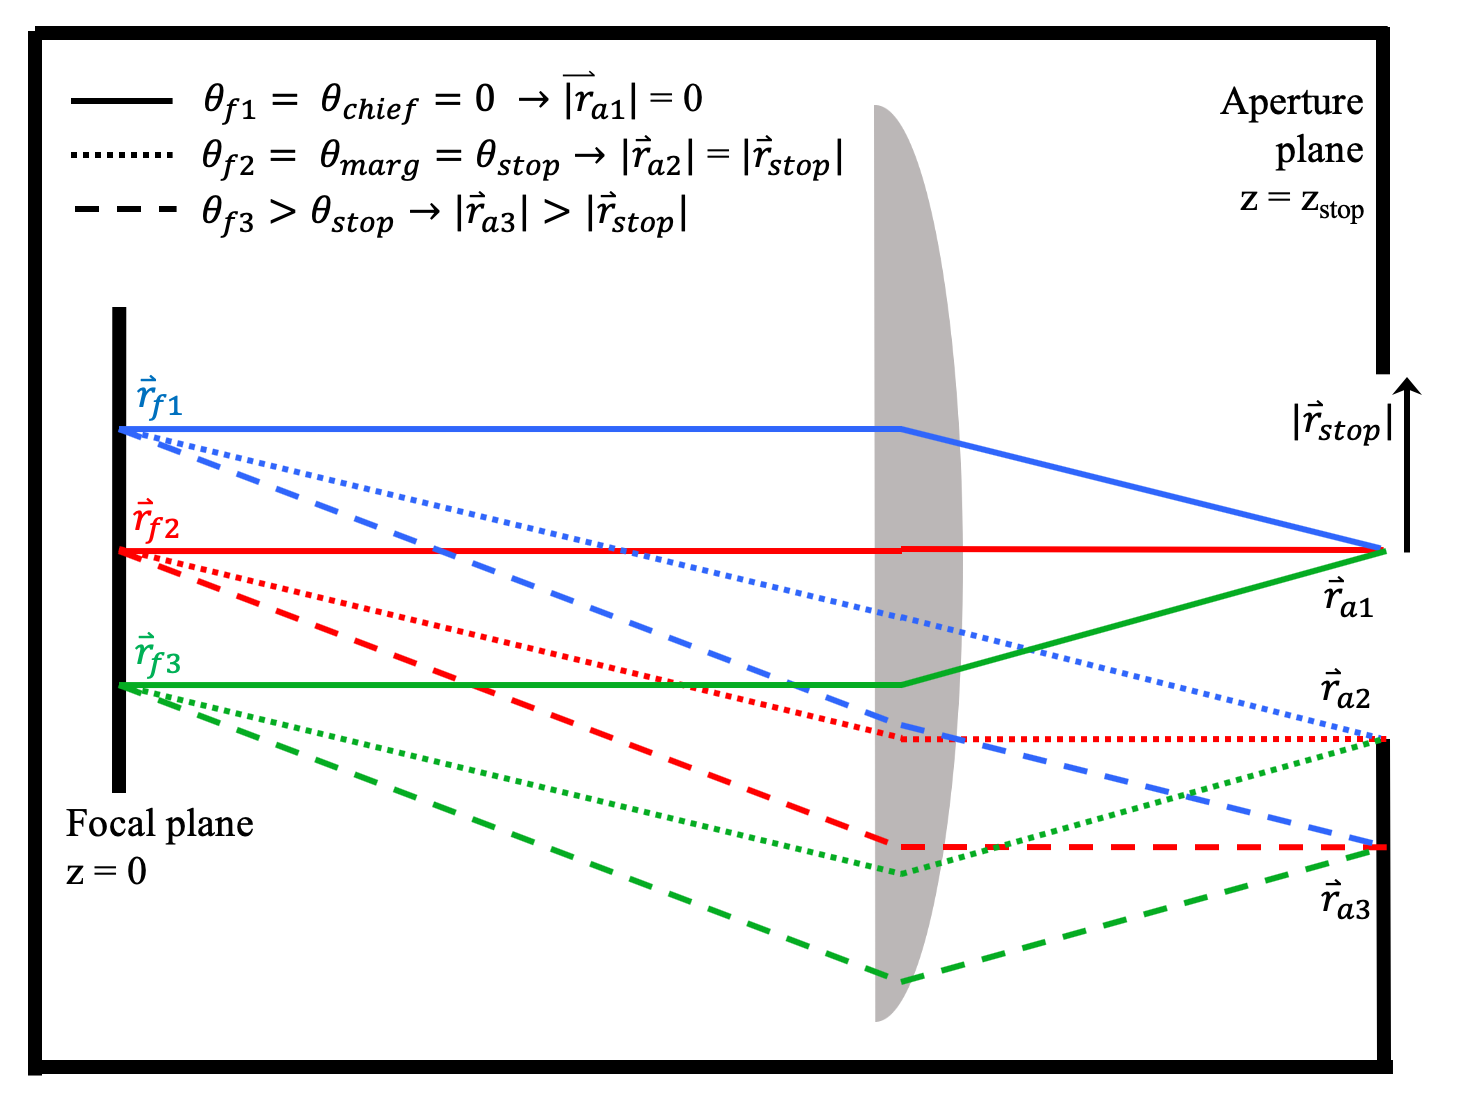
\includegraphics[width=0.55\linewidth, trim=0mm 0mm 0mm 0mm, clip=true]{WhiteNoiseCorrelations/Figures/simplified_optics_rays.png}
        }
    \caption[Simplified optical model assumed for calculating white-noise correlations]{\ref{fig:simple_optical_model:a} shows the behavior of an input plane wave into the assumed diffraction-limited optical system. The plane wave is truncated at the aperture stop and is focused as a spherical wave onto a diffraction-limited, single-moded detector pixel. \ref{fig:simple_optical_model:b} shows the behavior for off-axis pixels given the assumed idealized aperture stop. The pixel ray $(\theta_{fi}, \phi_{fi})$ is mapped injectively onto a corresponding location on the aperture stop $\vec{r}_{ai}$, and all rays from a single detector pixels are parallel at the aperture plane. A cross section where $\phi_{f} = 0$ is shown along with three special rays: the chief ray, the marginal ray, and a stopped ray.}
    \label{fig:simple_optics}
\end{figure}

\begin{figure}[!ht]
    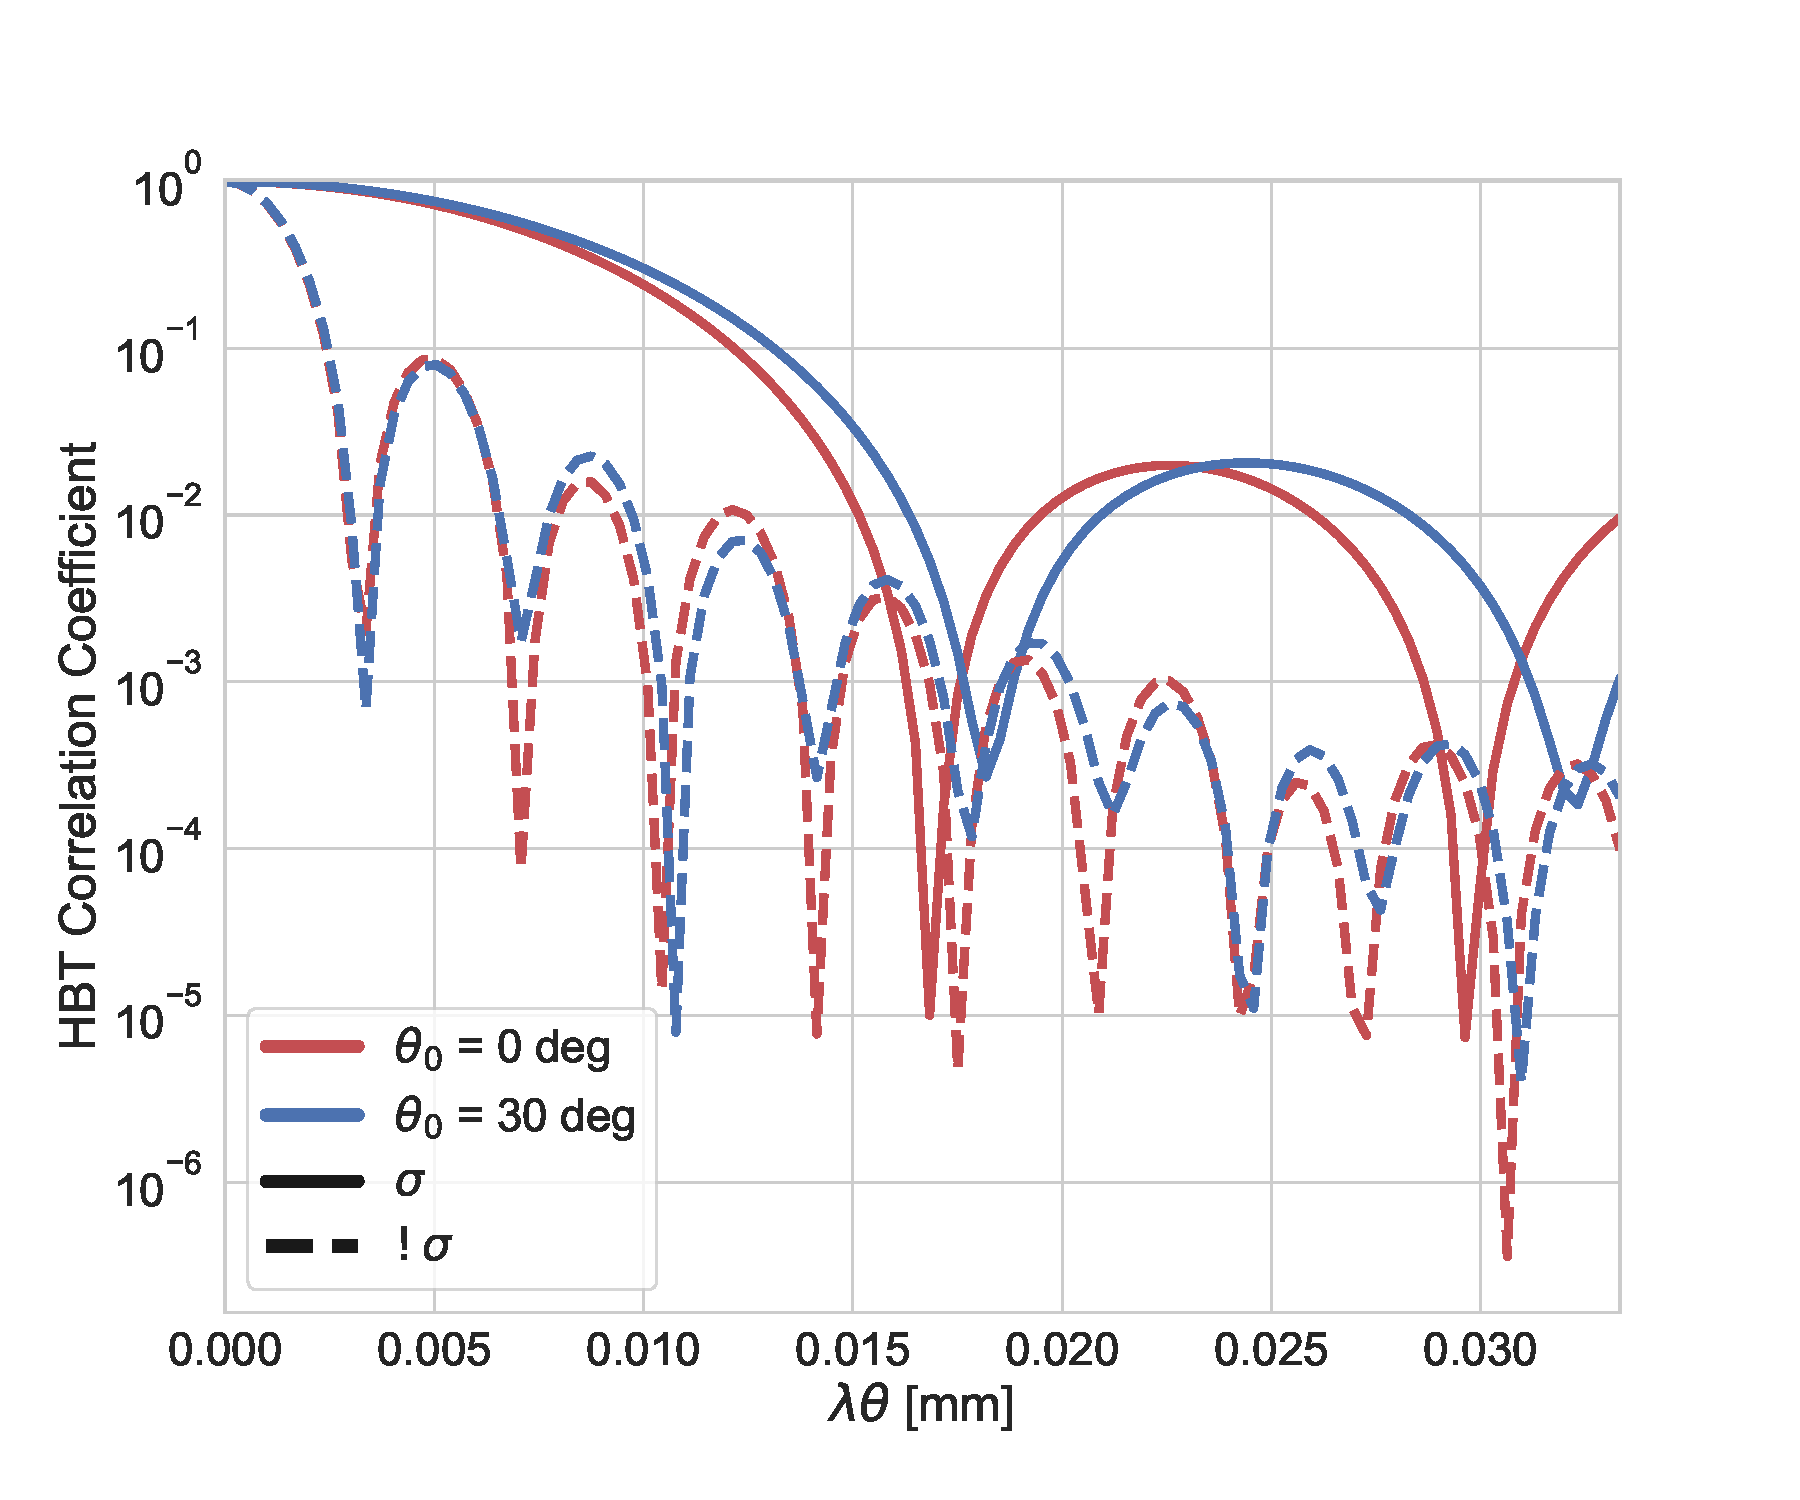
\includegraphics[width=\linewidth, trim=10mm 12mm 16mm 16mm, clip=true]{WhiteNoiseCorrelations/Figures/HBT_coeff.pdf}
    \caption[Hanbury Brown-Twiss correlation pattern on the focal plane]{The van Cittert-Zernike Fourier transform of a uniform intensity across a disk $\sigma$ and its inverse $\neg \sigma$ at the source plane, assuming the integration time is much longer than the coherence time. A non-zero viewing angle $\theta_{0}$ shifts power into the main lobe and widens the correlation pattern.}
    \label{fig:corr_geometry}
\end{figure}

\section{Pixel packing}

\begin{figure}
    \centering
    \subfloat[\label{fig:pixel_packing:a}]{
        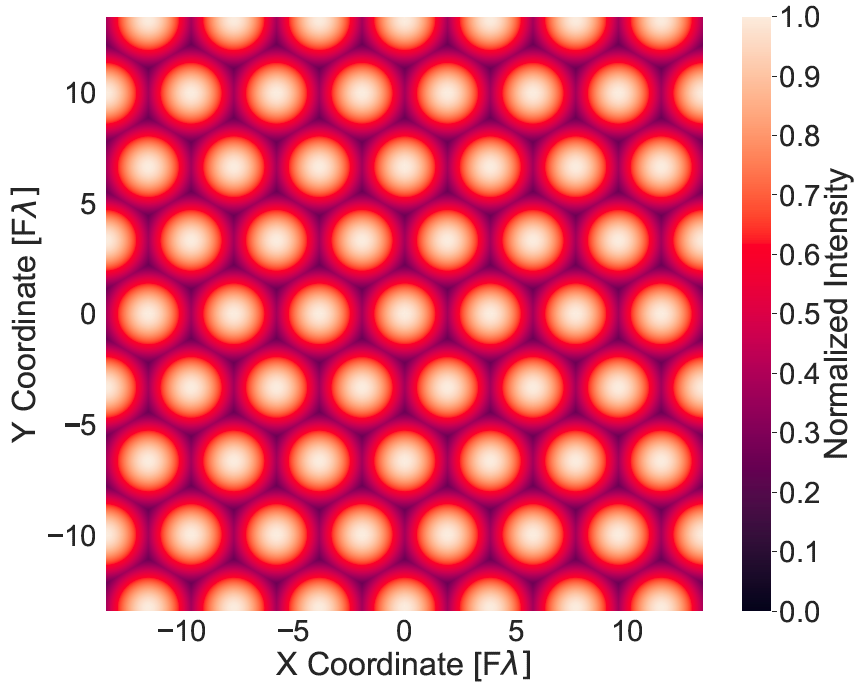
\includegraphics[width=0.40\linewidth, trim=0mm 0mm 0mm 0mm, clip=true]{WhiteNoiseCorrelations/Figures/2D_airy_screenshot.png}
        }
    \subfloat[\label{fig:pixel_packing:b}]{
        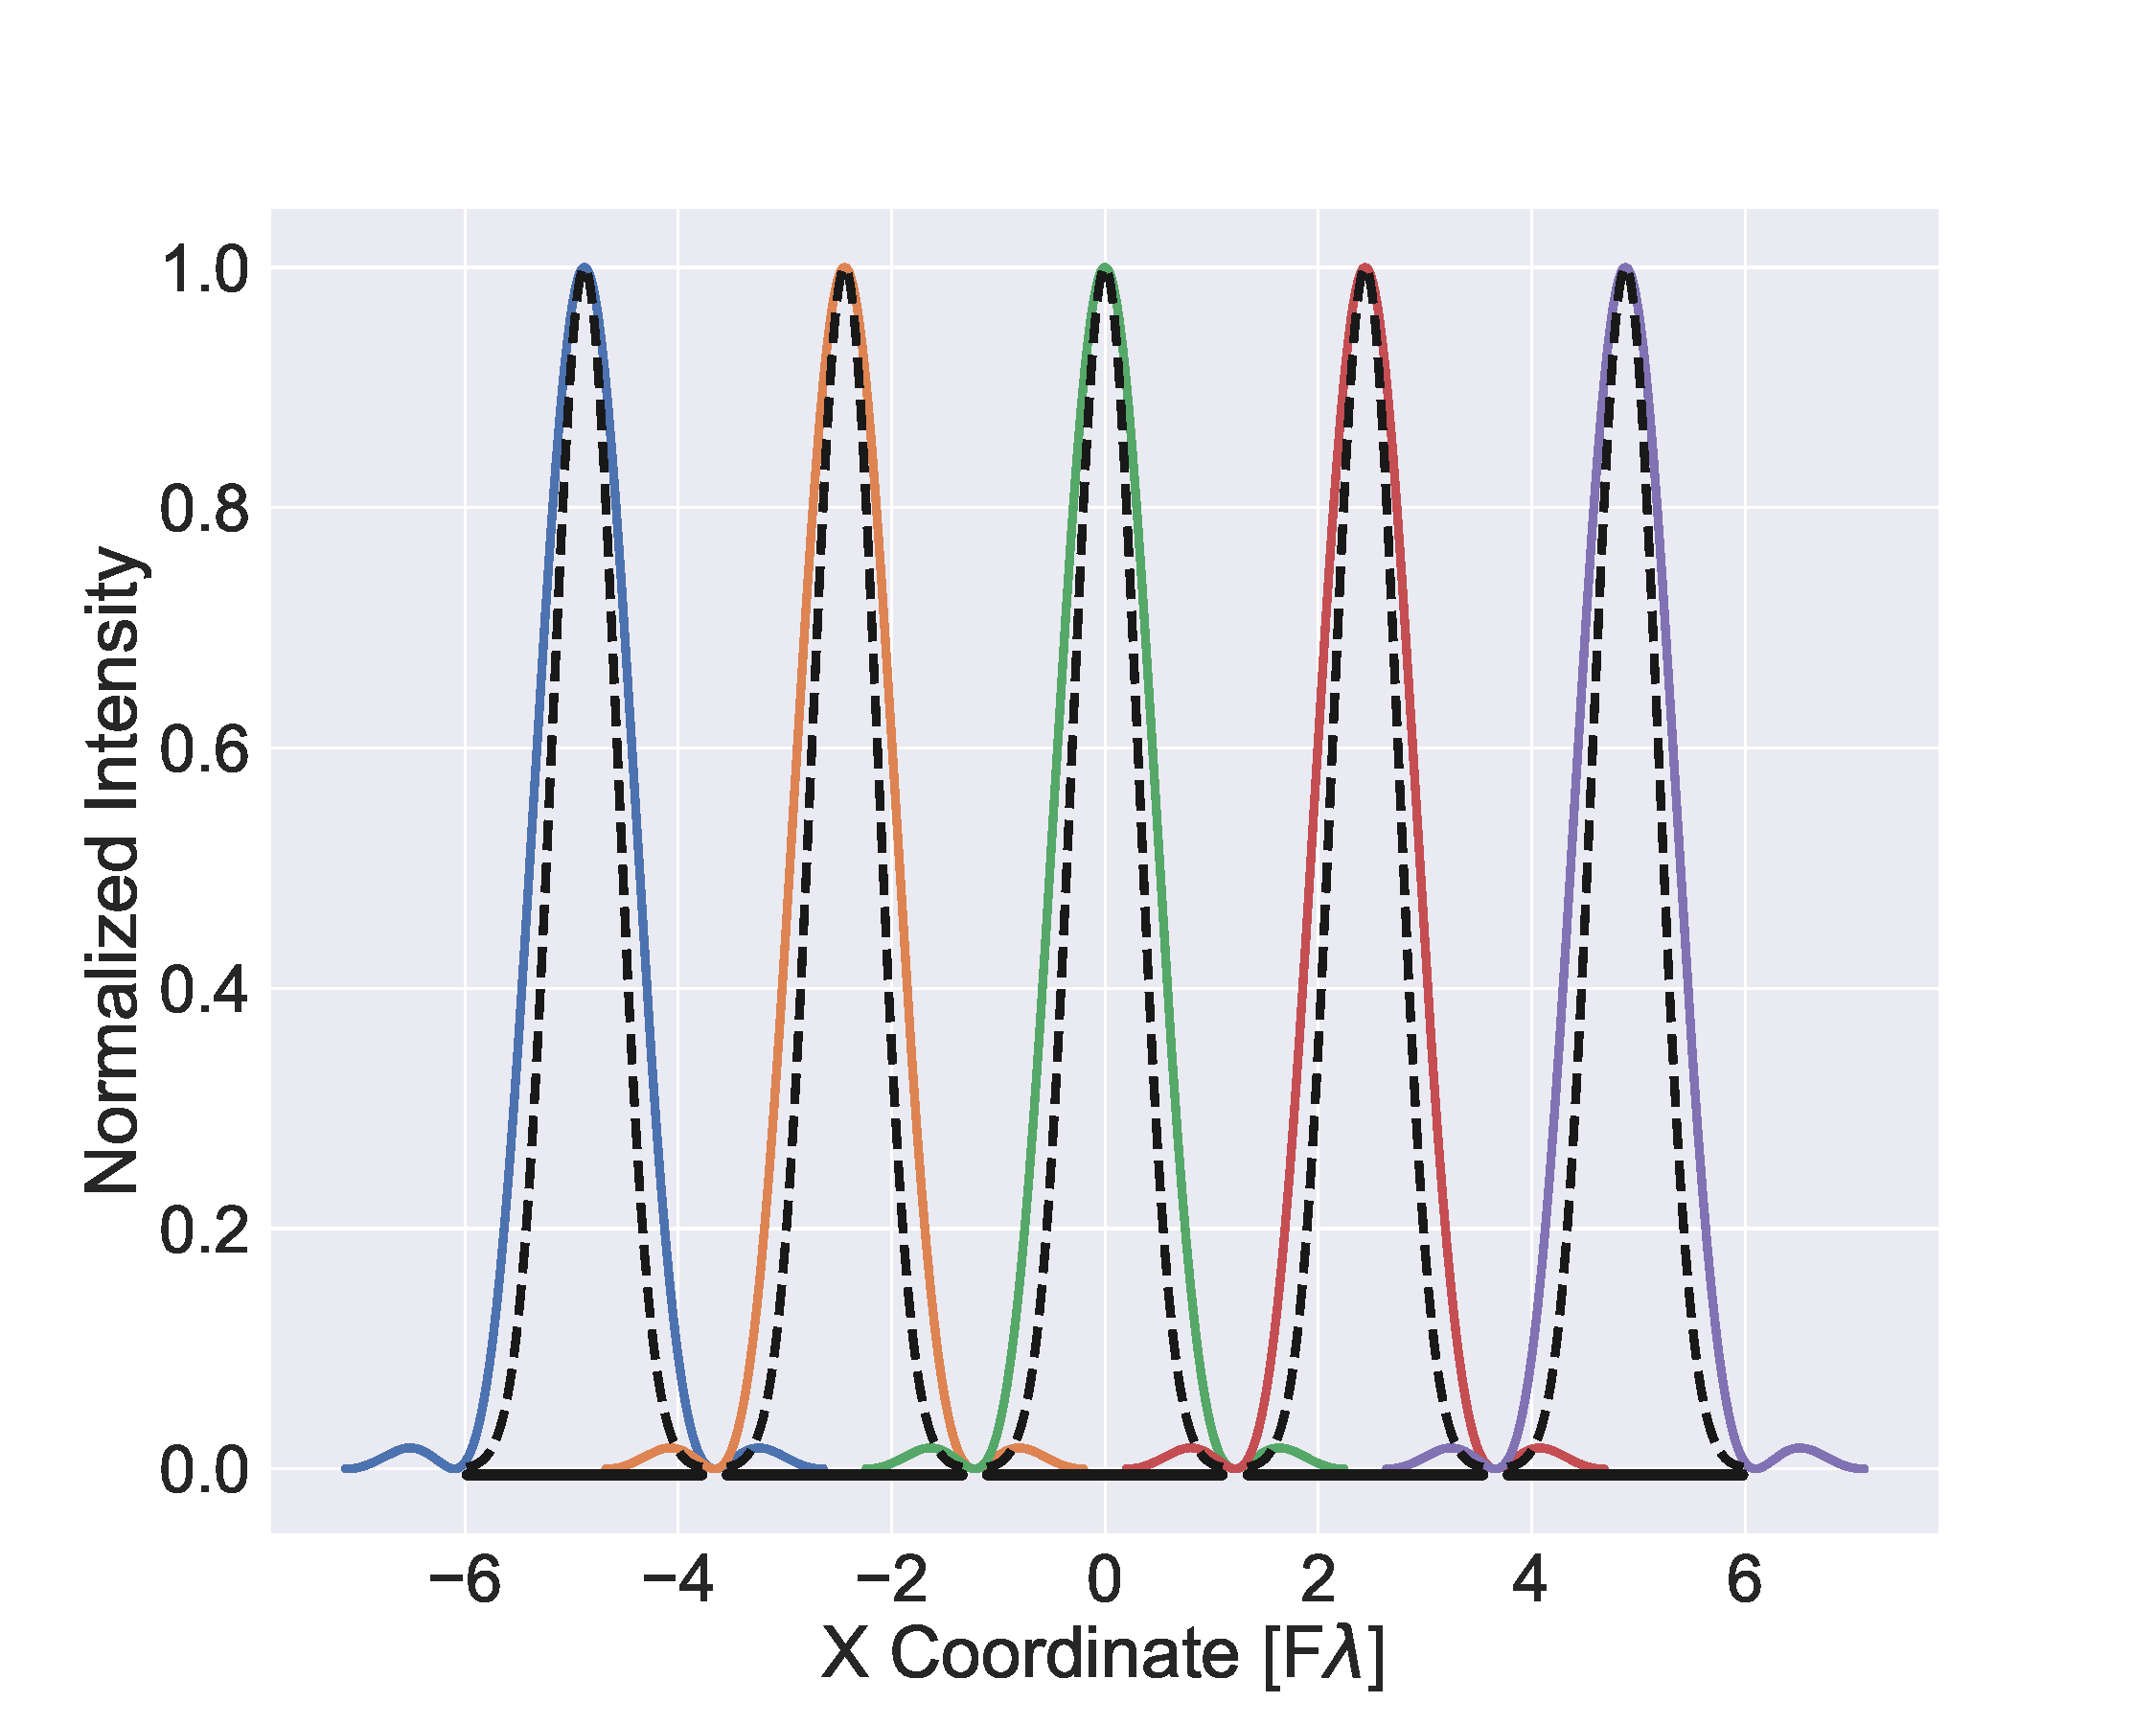
\includegraphics[width=0.55\linewidth, trim=0mm 0mm 0mm 0mm, clip=true]{WhiteNoiseCorrelations/Figures/1D_airy.pdf}
        }
    \caption[Contour diagram of independent spatial modes on the focal plane]{\ref{fig:pixel_packing:a} shows a hex-packed array of independent modes imaged onto a plane by an aperture-objective system. Each Airy disk is spaced $1.22 F \lambda$ from its neighbors. \ref{fig:pixel_packing:b} shows a 1D cut of the independent spatial modes, overlaid with an example detector pixel packing of one pixel per Airy disk. The Gaussian beam from a typical corrugated horn from the shown pixel size is shown with a dotted line.}
    \label{fig:pixel_packing}
\end{figure}

\begin{figure}[!ht]
    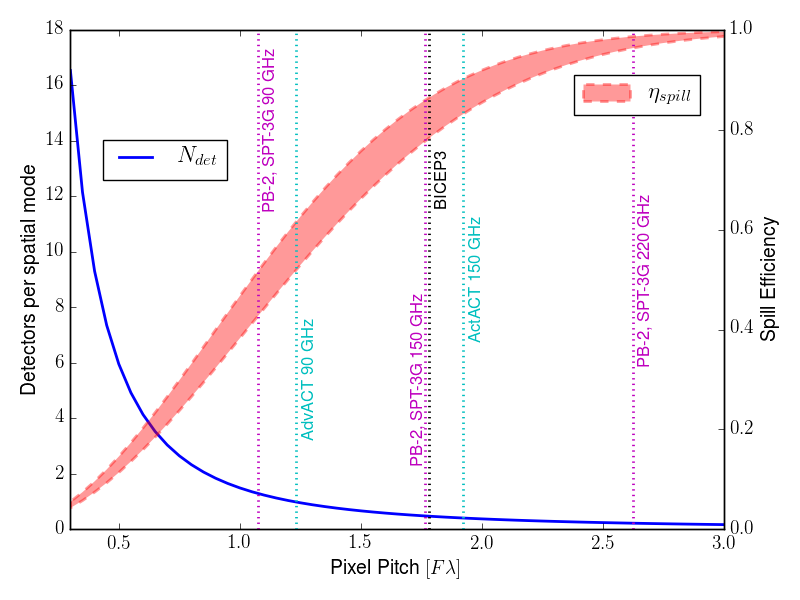
\includegraphics[width=\linewidth]{WhiteNoiseCorrelations/Figures/stopEff_Ndet.png}
    \caption[Detectors per spatial mode and spill efficiency vs pixel pitch, along with the value from various experiments]{Detectors per spatial mode and spill efficiency vs pixel pitch, along with the value from various experiments. The blue line shows the number of detectors per spatial mode, the red shaded region shows the range of possibilities for stop spillover efficiency, which depends on the antenna illumination area, and the vertical dotted lines show the location on these curves for various existing experiments. All fielded focal planes tend to pack $\sim$ 1 pixel per spatial mode, which gives a high spillover effieicncy. However, as developing detector fabrication techniques allow for denser focal planes, future experiments, such as Simons Observatory, plan to pack more densely, making a precise characterization of white-noise correlations important to an accurate array sensitivity estimate.}
    \label{fig:field_flambda_spacing}
\end{figure}